\documentclass[]{spie}
\usepackage[utf8]{inputenc}
\usepackage{graphicx}
\usepackage{amsmath,amsfonts,amssymb}
\usepackage[colorlinks=true, allcolors=blue]{hyperref}
\usepackage{booktabs}

\renewcommand{\baselinestretch}{1.0} % Change to 1.65 for double spacing

\title{Comparative Study of SRCNN and ESRGAN for Remote Sensing Image Super-Resolution on the Satellite Image Caption Generation Dataset}

\author[a]{Harshdeep Singh}
\affil[a]{Sri Guru Granth Sahib World University, Fatehgarh Sahib, India}

\authorinfo{Further author information: (Send correspondence to H.S.)\\H.S.: E-mail: harsh0129h@gmail.com}

\pagestyle{empty}
\setcounter{page}{1}

\begin{document}

\maketitle

\begin{abstract}
Super-resolution (SR) is crucial in remote sensing, where satellite image quality impacts land-use analysis, object detection, and caption generation. This paper compares the Super-Resolution Convolutional Neural Network (SRCNN) and Enhanced Super-Resolution Generative Adversarial Network (ESRGAN) on the Kaggle \textit{Satellite Image Caption Generation} dataset. Low-resolution inputs were generated via bicubic downsampling ($\times2$ and $\times4$). Reconstructions were evaluated against standardized 256$\times$256 ground truth images using Structural Similarity Index Measure (SSIM) and Peak Signal-to-Noise Ratio (PSNR). Results show ESRGAN consistently outperforms SRCNN, especially in texture-rich scenes, by producing sharper details and higher perceptual fidelity. This study highlights the role of GAN-based SR models for enhancing satellite imagery quality.
\end{abstract}

\keywords{Super-resolution, SRCNN, ESRGAN, Satellite Imagery, SSIM, PSNR, Remote Sensing}

% -----------------------------
\section{INTRODUCTION}
% -----------------------------
Satellite imagery plays a vital role in remote sensing tasks such as land-use classification, environmental monitoring, and language-based caption generation. However, sensor limitations, atmospheric interference, and storage constraints often lead to low-resolution (LR) imagery that lacks fine textural and structural details. Image super-resolution (SR) aims to reconstruct high-resolution (HR) images from LR inputs, thereby enhancing interpretability and downstream task performance.

Traditional methods, such as nearest-neighbor, bilinear, and bicubic interpolation, are fast but cannot reconstruct missing high-frequency content, leading to blurred outputs and smoothed edges. Deep learning-based SR has changed this landscape: CNN models like SRCNN \cite{dong2014learning} demonstrated the feasibility of learning an LR-to-HR mapping directly from data, while GAN-based methods like SRGAN \cite{ledig2017srgan} and ESRGAN \cite{wang2018esrgan} enhanced perceptual realism via adversarial and perceptual losses.

This work conducts a controlled comparison of SRCNN and ESRGAN using a standardized SR evaluation protocol on the Kaggle \textit{Satellite Image Caption Generation} dataset \cite{kaggle_dataset}. We evaluate both $\times2$ and $\times4$ upscaling using SSIM (primary) and PSNR (secondary), with careful attention to color handling, normalization, and image pairing. Quantitative findings are complemented by qualitative side-by-side panels and patch zooms.

\subsection{Importance of SR in Remote Sensing}
High-quality SR benefits:
\begin{itemize}
    \item \textbf{Urban Planning:} Clearer road networks, roofs, and boundaries enable improved mapping and infrastructure planning.
    \item \textbf{Agriculture:} Better crop texture and field boundaries aid monitoring, irrigation optimization, and yield estimation.
    \item \textbf{Disaster Response:} Faster and more accurate damage assessment depends on recognizable object-level details.
    \item \textbf{Environmental Monitoring:} Tracking deforestation, coastline changes, and water bodies requires spatial detail beyond raw LR.
\end{itemize}

\subsection{Limitations of Interpolation-Based Upscaling}
Interpolation methods do not invent new information and cannot reconstruct lost high frequencies. Outputs tend to be smooth with poor edge definition, limiting performance in tasks requiring crisp boundaries and textural cues.

\subsection{Advances in Deep Learning for SR}
\textbf{SRCNN} \cite{dong2014learning} introduced an end-to-end CNN with three convolutional stages (patch embedding, non-linear mapping, reconstruction).  
\textbf{ESRGAN} \cite{wang2018esrgan} uses RRDBNet, a deeper residual-in-residual dense block network, with relativistic GAN loss and perceptual loss to reconstruct sharp, realistic textures. GAN-based SR is known to provide high perceptual quality that aligns better with human vision for complex textures.

% -----------------------------
\section{DATASET}
% -----------------------------
We use the Kaggle \textit{Satellite Image Caption Generation} dataset \cite{kaggle_dataset}, which provides a diverse collection of RGB satellite images spanning urban, vegetation, water bodies, deserts, and farmland. Although the dataset was originally curated for image captioning, its variety and visual complexity make it apt for SR assessment.

\subsection{Preprocessing and Standardization}
To ensure consistent evaluation:
\begin{itemize}
    \item \textbf{HR Ground Truth:} All selected images were standardized to 256$\times$256 resolution and converted to \texttt{PNG} to avoid JPEG compression artifacts.
    \item \textbf{LR Inputs:} LR images were generated via bicubic downsampling (OpenCV) at $\times2$ (128$\times$128) and $\times4$ (64$\times$64).
    \item \textbf{Naming and Pairing:} Filenames were normalized so that HR and predictions align by stem name. Evaluation scripts strip suffixes like \texttt{\_x2}, \texttt{\_x4}, \texttt{\_rlt}, and method tags for robust pairing.
\end{itemize}

\subsection{Directory Structure}
\begin{itemize}
  \item \texttt{data/processed/HR/} – Ground truth 256$\times$256 PNGs.
  \item \texttt{data/processed/LR\_x2/}, \texttt{LR\_x4/} – Bicubic LR inputs.
  \item \texttt{results/SRCNN\_x2/}, \texttt{results/SRCNN\_x4/}, \texttt{results/ESRGAN\_x2/}, \texttt{results/ESRGAN\_x4/}.
  \item \texttt{results/visuals/} – Generated plots and panels.
  \item \texttt{eval\_results.csv} – Per-image metrics (SSIM/PSNR).
\end{itemize}

\subsection{Sanity Checks}
Before metric computation, we validate:
\begin{enumerate}
    \item Each prediction has an HR match by stem name.
    \item Each prediction is RGB; channel ordering is consistent.
    \item Shapes match HR (256$\times$256); otherwise, we resize with bicubic for metric stability.
\end{enumerate}

% -----------------------------
\section{METHODOLOGY}
% -----------------------------
\subsection{Models}
\textbf{SRCNN} \cite{dong2014learning}: A 3-layer CNN with patch embedding, non-linear mapping (ReLU), and reconstruction. Used as a strong, simple CNN baseline; implemented in PyTorch with pretrained weights.

\textbf{ESRGAN} \cite{wang2018esrgan}:
\begin{itemize}
    \item \textbf{Backbone:} RRDBNet (Residual-in-Residual Dense Blocks) to enable deep feature reuse and stable training.
    \item \textbf{Losses:} Relativistic GAN (RaGAN) and VGG-based perceptual loss to sharpen textures and improve realism.
    \item \textbf{Weights:} Pretrained RRDB\_ESRGAN\_x4 weights (official implementation).
\end{itemize}

\subsection{Inference Setup}
\begin{itemize}
  \item \textbf{SRCNN:} Upscales LR inputs and outputs are aligned to 256$\times$256 during evaluation.
  \item \textbf{ESRGAN:} Directly upsamples LR to HR (e.g., 64$\rightarrow$256 at $\times4$).
  \item All outputs saved to \texttt{results/\{METHOD\}\_\{scale\}} with consistent stems.
\end{itemize}

\subsection{Evaluation Protocol}
We compute SSIM and PSNR for each prediction against its HR counterpart:
\begin{itemize}
  \item \textbf{SSIM:} Computed in \underline{RGB}, with \texttt{channel\_axis=2} and \texttt{data\_range=1.0} on normalized floats \cite{scikit_image, geeksforgeeks_similarity}.
  \item \textbf{PSNR:} Computed from MSE with \texttt{data\_range=1.0} \cite{scikit_image, geeksforgeeks_psnr}.
    \item \textbf{Aggregation:} Per-image CSV; grouped means by class/method/scale; overall means for headline results.
\end{itemize}

\subsection{Qualitative Assessment}
We include:
\begin{itemize}
    \item \textbf{Side-by-side panels:} LR $\rightarrow$ SRCNN $\rightarrow$ ESRGAN $\rightarrow$ HR.
    \item \textbf{Patch zooms:} Crops over edges/texture regions (roofs, roads, vegetation).
    \item \textbf{Difference maps:} $|$HR $-$ Prediction$|$ to highlight residual errors and structural mismatches.
\end{itemize}

\subsection{Hardware and Runtime}
Experiments run on a GPU-enabled environment (e.g., NVIDIA RTX-class GPU). Inference is real-time for SRCNN and near-real-time for ESRGAN given 256$\times$256 HR targets. Evaluation is implemented in Python with OpenCV, NumPy, scikit-image, and pandas.

\subsection{Reproducibility}
The full pipeline (data prep, model inference, metrics, and plots) is scripted in the repository \cite{github_repo}. The evaluation script ensures deterministic pairing and uniform preprocessing.

% -----------------------------
\section{RESULTS \& DISCUSSION}
% -----------------------------
\subsection{Quantitative Results}
Table~\ref{tab:overall_performance} summarizes the overall means across all evaluated images. Values are computed from the exported CSV and align with the standardized protocol.

\begin{table}[h!]
\centering
\caption{Overall Mean SSIM and PSNR (higher is better).}
\label{tab:overall_performance}
\begin{tabular}{llll}
\toprule
\textbf{Scale} & \textbf{Method} & \textbf{SSIM} & \textbf{PSNR (dB)} \\
\midrule
$\times2$ & SRCNN  & 0.693 & 25.03 \\
$\times2$ & ESRGAN & 0.837 & 29.92 \\
$\times4$ & SRCNN  & 0.409 & 20.95 \\
$\times4$ & ESRGAN & 0.644 & 25.91 \\
\bottomrule
\end{tabular}
\end{table}

ESRGAN consistently outperforms SRCNN across both scales, with larger margins at $\times4$. The SSIM gains reflect ESRGAN's ability to reconstruct fine structure and sharp textures, which is consistent with GAN-based perceptual optimization.

\subsection{Per-Class Analysis}
Texture-rich categories (e.g., urban/residential, forests, farmland) show stronger ESRGAN advantages due to complex edge/texture reconstruction. Smoother categories (e.g., deserts, bareland) show smaller margins and, in rare cases, similar PSNR between methods.

\begin{figure}[h!]
\centering
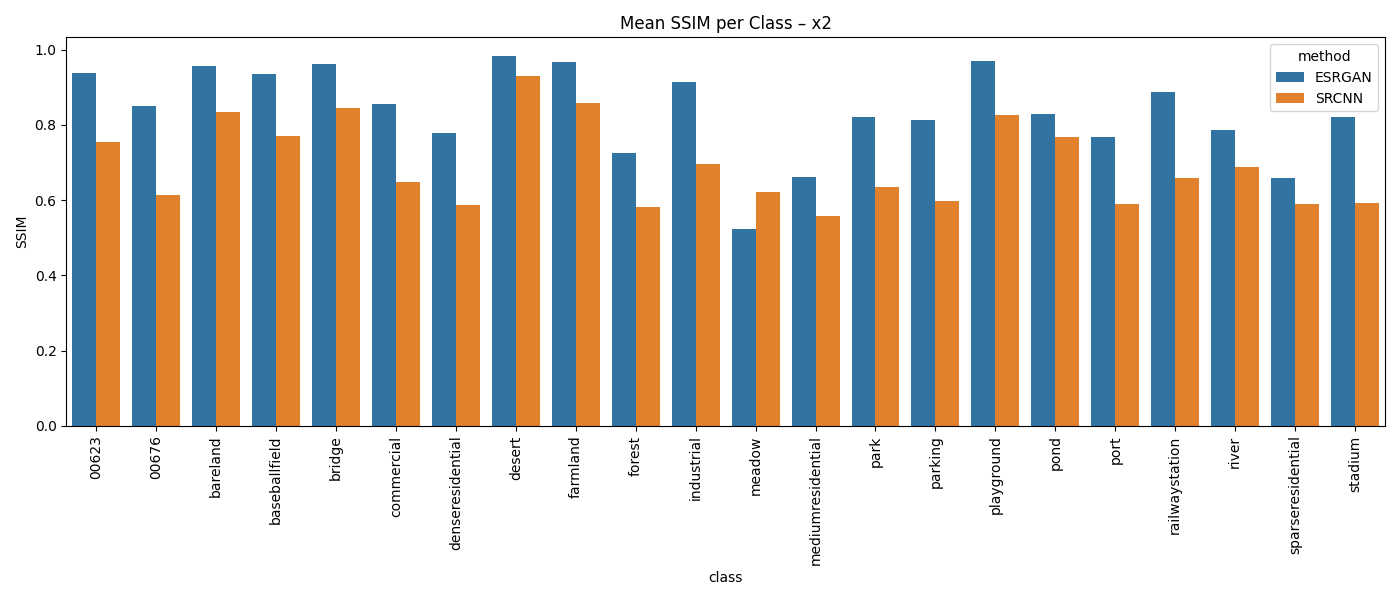
\includegraphics[width=0.85\textwidth]{ssim_per_class_x2.png}
\caption{Mean SSIM per class at $\times2$ for SRCNN vs ESRGAN.}
\label{fig:ssim_x2}
\end{figure}

\begin{figure}[h!]
\centering
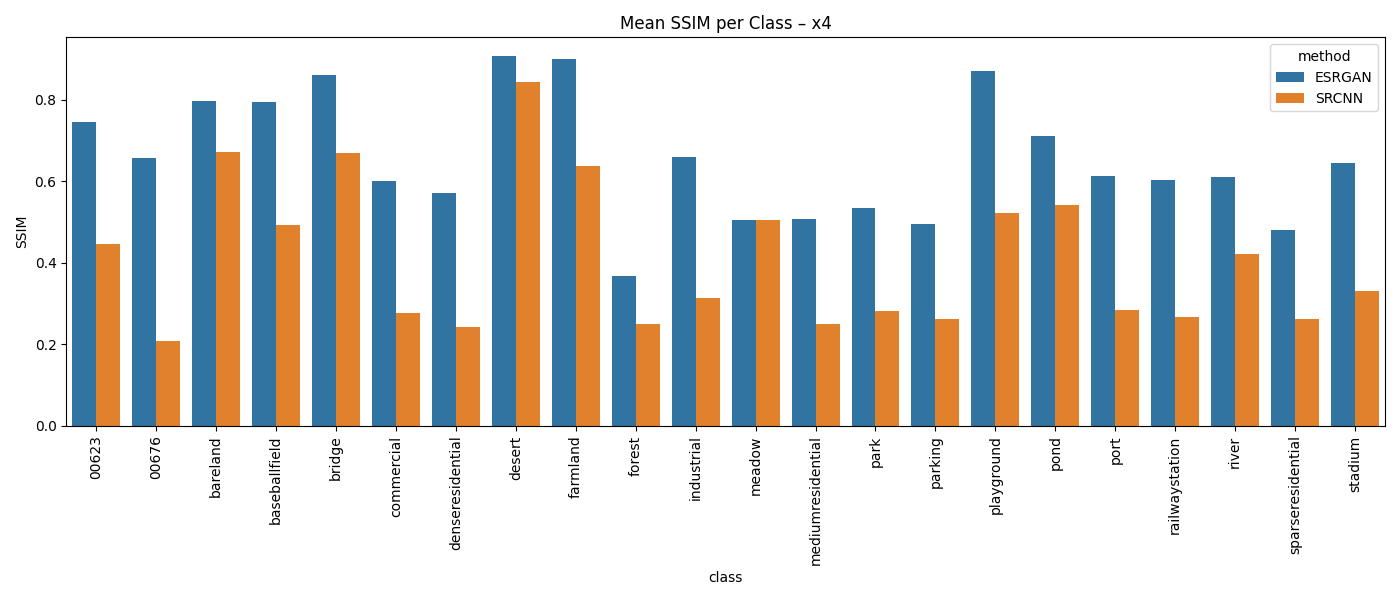
\includegraphics[width=0.85\textwidth]{ssim_per_class_x4.png}
\caption{Mean SSIM per class at $\times4$ for SRCNN vs ESRGAN.}
\label{fig:ssim_x4}
\end{figure}

\subsection{Delta SSIM Distribution}
The histogram of $\Delta$SSIM $=$ SSIM(ESRGAN)$-$SSIM(SRCNN) shows a right-skewed distribution, indicating consistent improvements by ESRGAN across the majority of samples.

\begin{figure}[h!]
\centering
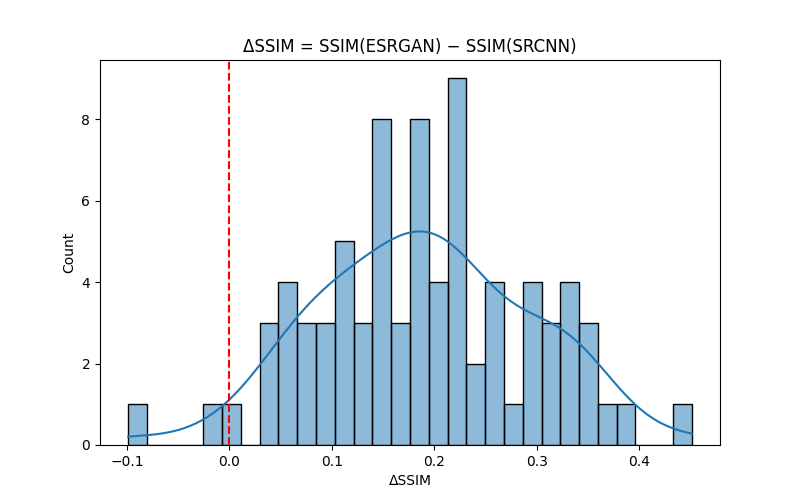
\includegraphics[width=0.8\textwidth]{delta_ssim_hist.png}
\caption{Distribution of $\Delta$SSIM (ESRGAN minus SRCNN) across all images.}
\label{fig:delta_ssim}
\end{figure}

\subsection{Qualitative Comparisons}
Figure~\ref{fig:side_by_side} shows a representative comparison panel. ESRGAN produces crisper edges and well-defined small structures (e.g., rooftops, roads), while SRCNN tends to oversmooth textures. Additional panels and zoomed patches are provided in the repository.

\begin{figure}[h!]
\centering
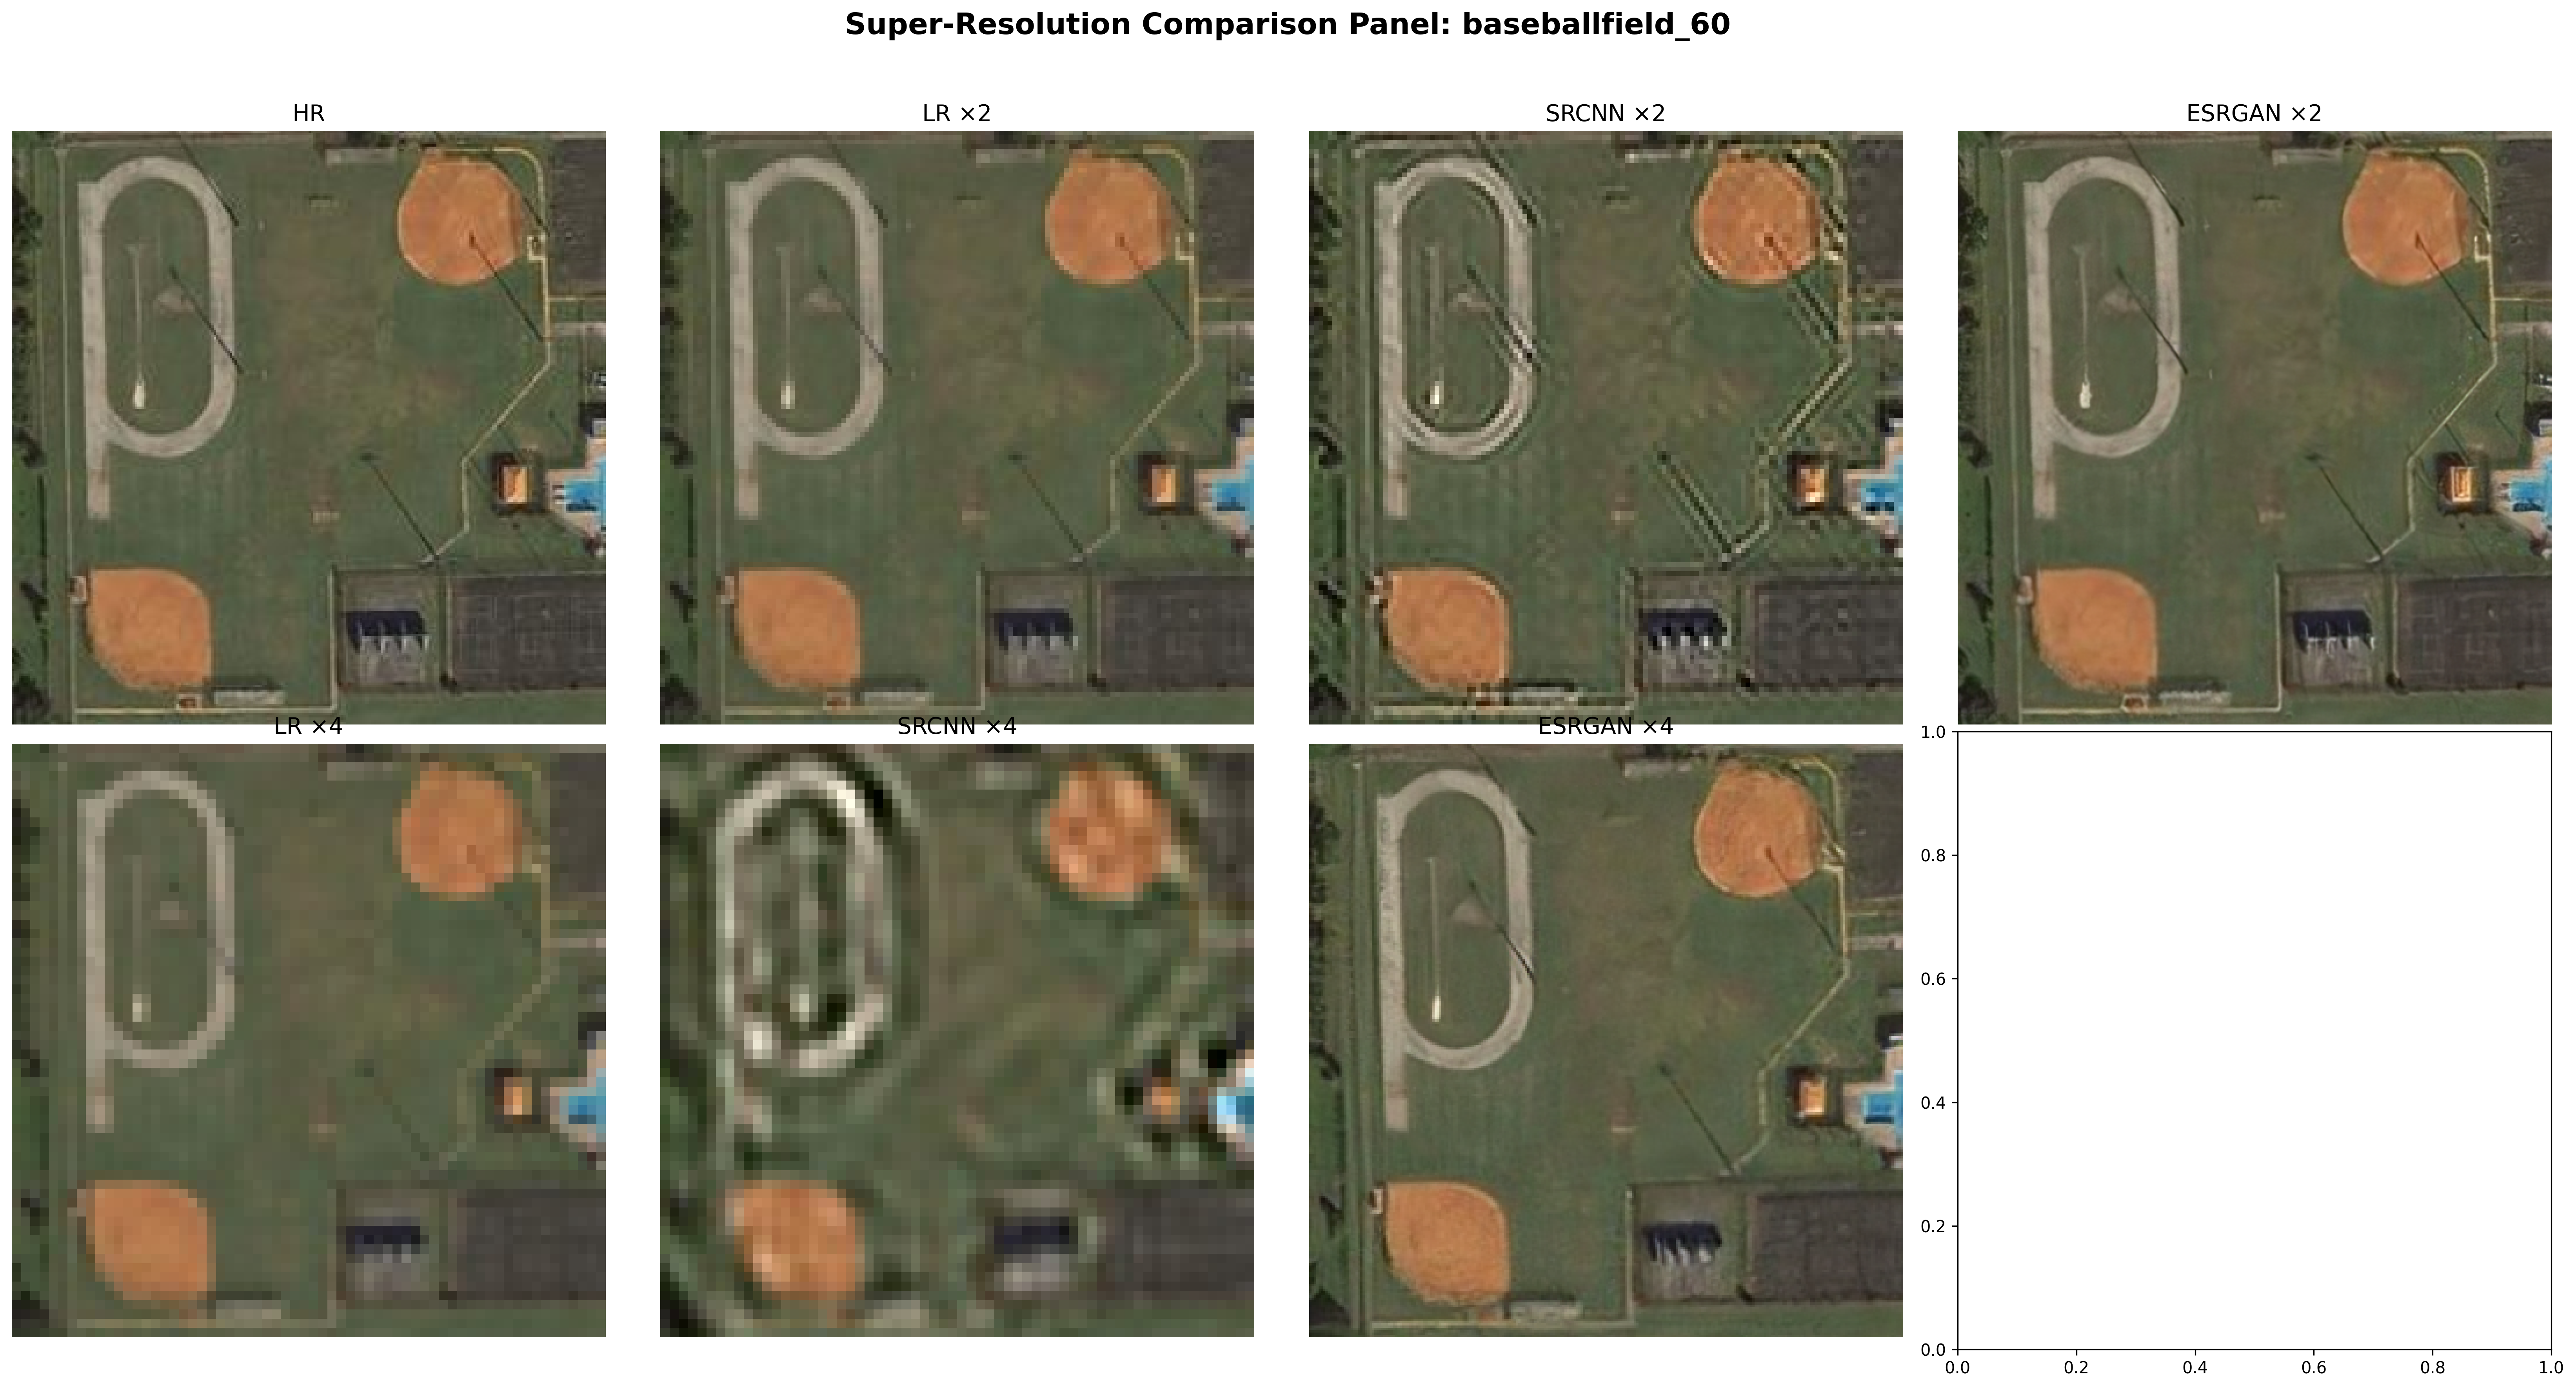
\includegraphics[width=0.92\textwidth]{baseballfield_60_panel.png}
\caption{Representative side-by-side comparison (left to right): LR input, SRCNN, ESRGAN, HR ground truth.}
\label{fig:side_by_side}
\end{figure}

\subsection{Discussion}
\textbf{SSIM vs PSNR:} While PSNR improves with ESRGAN, SSIM captures perceptual quality differences more effectively, especially over textured regions.  
\textbf{Scale Sensitivity:} Both methods degrade at $\times4$, but ESRGAN remains more robust.  
\textbf{Use Cases:} ESRGAN is favorable for applications relying on human interpretability and texture fidelity; SRCNN may suffice where smoother outputs and lower compute cost are acceptable.

% -----------------------------
\section{CONCLUSION}
% -----------------------------
We presented a comparative study of SRCNN and ESRGAN for SR on the Kaggle \textit{Satellite Image Caption Generation} dataset. Using a standardized evaluation protocol (bicubic degradation, RGB SSIM with channel-aware configuration, and PSNR on normalized floats), we showed that ESRGAN delivers superior structural and perceptual quality across $\times2$ and $\times4$ scales. Visual assessments corroborate quantitative gains.

Future work includes adding perceptual metrics (LPIPS, FID), exploring remote-sensing–specific SR models, and scaling to larger multi-sensor datasets. All scripts, metrics, and figures are available in the project repository \cite{github_repo} for full reproducibility.

\bibliographystyle{spiebib}
\bibliography{references}

\appendix
\section{Reproducibility Details}
All preprocessing, inference, and evaluation code is available in our GitHub repository \cite{github_repo}. For clarity, we summarize the exact commands:

\subsection{SRCNN Inference}
\begin{verbatim}
python test_srcnn.py \
  --model models/srcnn.pth \
  --input data/processed/LR_x2 \
  --output results/SRCNN_x2
\end{verbatim}

\subsection{ESRGAN Inference}
\begin{verbatim}
python test.py \
  --model models/RRDB_ESRGAN_x4.pth \
  --input data/processed/LR_x4 \
  --output results/ESRGAN_x4
\end{verbatim}

\subsection{Evaluation}
\begin{verbatim}
python evaluate_models.py \
  --hr data/processed/HR \
  --pred results \
  --out eval_results.csv
  
\end{verbatim}


\end{document}

